\documentclass[11pt, oneside]{amsart}
%\documentclass[11pt]{article}
%\usepackage[top =2.8cm, bottom=2.8cm, left=2.8cm, right=2.8cm]{geometry}
\usepackage{geometry}
\geometry{letterpaper}
\usepackage[english]{babel}
\usepackage[utf8]{inputenc}
\usepackage{graphicx}
\usepackage{float}
\usepackage{etex,mathtools}
\usepackage{amssymb}
\usepackage{enumitem}
\usepackage{amsmath}
\usepackage{caption}
\usepackage{listings}
\usepackage{array}
\usepackage{cite}
\graphicspath{{images/}}
\usepackage[colorinlistoftodos]{todonotes}

\newif\ifnotesw \noteswtrue
\newcommand{\notes}[1]{\ifnotesw \textcolor{red}{  $\clubsuit$\ {\sf \bf \it  #1}\ $\clubsuit$ }\fi}
\newcommand{\given}{\mathbin{\vert}}

\title[]{Project report, PGM}
%\title{Project report, PGM}

\author[1]{Nicolas Jouvin}
\author[2]{Thomas Kerdreux}
\author[3]{Louis Thiry}
%\author{Louis Thiry \and Thomas Kerdreux \and Nicolas Jouvin}

\begin{document}
\bibliographystyle{unsrt}

\maketitle

\section*{introduction}

This article presents an algorithm to learn non-linear stochastic dynamical system with incomplete observation.
It can be applied only for a specific parametrization of non-linear functions.
This algorithm is an instance of EM algorithm, estimmating the non-observed variables in the E-Step and learning the parameters of the non-linear functions in the M-Step.

It is regrettable that none of the computations that are necessary for the implementations of the presented algorihtm are fully presented, neither for the E-Step nor for the M-Step.
This article is the sixth chapter of the book "Kalman Filtering and Neural Network" edited by Simon Haykin and the authors mention the chapter one for some of the computations they do not provide.
We luckily found on the internet a numerical version of that book (which is otherwise available for sale for more than 100 euros) and we found out that the graphical model that the authors use in the article is even not same as the one presented in chapter one of that book.

So before summerizing this article, we wan't to insist on the fact that we were really disapointed by the quality of that article that spends a lot of time explaining simple things (EM algorithm principle, linear Kalman filter equations) but that provide none of the key computations, neither for the E-Step (Extended Kalman Smoothing) nor for the M-Step (log likelihood maximization).

It costed us a lot of time and reflexion to understand that we had to do it, and then to do it.
Fortunatelly, the lecture notes were of great help in that work.


\section{The model}

This article deals with a non-linear stochastic dynamical system in discrete-time.
The authors model with this systems with five sequences :
\begin{itemize}
  \item $(x_t)_{t=1 \ldots T}$ (in $\mathbb{R}^p$) are called the \textbf{states} and are \textbf{unknown}.
  \item $(u_t)_{t=1 \ldots T}$ (in $\mathbb{R}^q$) are called the \textbf{inputs} and are \textbf{observed}.
  \item $(y_t)_{t=1 \ldots T}$ (in $\mathbb{R}^n$) are called the \textbf{outputs} and are \textbf{observed}.
  \item $(v_t)_{t=1 \ldots T-1}$ and $(w_t)_{t=1 \ldots T}$ (in $\mathbb{R}^p \times \mathbb{R}^n$) are zero-mean \textbf{Gaussian iid noises} of covariance matrices $Q \in \mathbb{R}^{p \times p}$ and $R \in \mathbb{R}^{n \times n}$, and are unknown.
\end{itemize}
and with two \textbf{non-linear differentiable} functions :
\begin{align*}
  f \colon \mathbb{R}^p \times \mathbb{R}^q &\to \mathbb{R}^p\\
  (x,u) &\mapsto f(x, u)\\
  g \colon \mathbb{R}^p \times \mathbb{R}^q &\to \mathbb{R}^n\\
  (x,u) &\mapsto g(x, u)\\
\end{align*}

The stochastic dynamics equations are:
\begin{eqnarray}
  x_{t+1}&=& f(x_t,u_t)+v_t\label{eq:A}\\
  y_t &=& g(x_t,u_t)+w_t\label{eq:B}
\end{eqnarray}
This system can be represented with the graphical model:
\begin{figure}[H]
	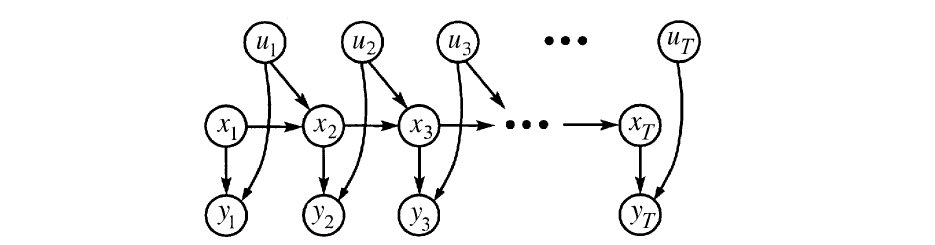
\includegraphics[width=14cm]{screenshot_graphical_model.PNG}
	\captionof{figure}{Graphical model of our system.}
\end{figure}


\bibliographystyle{plain}
\section{Presented algorithm}

The goal of the algorithm presented in this article is to learn the dynamics of the system, which means learn the functions $f$ and $g$  and the covariance matrices $Q$ and $R$ that are supposed to be unknown.
The functions $f$ and $g$ are parametrized by $\theta_f$ and $\theta_g$.

So our dynamical system is prametrized by $\theta = \left(\theta_f, \theta_g, Q, R \right)$ and we want to learn the value of $\theta$ with the maximum likelihood principle.

The complication is that both the parameter $\theta$ and the state sequence $(x_t)_{t=1 \cdots T}$ are unknown.
In such case where both states and parameters are unknown, a typical approach is to use an iterative Expectations Maximization (EM) algorithm:
\begin{itemize}
  \item we begin with inital values for the parameter $\theta^{(0)} = \left( \theta_f^{(0)}, \theta_g^{(0)}), Q^{(0)}, R^{(0)} \right)$.
\item For $k=1 \ldots K$, we itertate E-step and M-step:
  \begin{itemize}
    \item In the \textbf{E-step}, the states $(x_t)_{t=1 \cdots T}$ are inferred (or estimated) knowing the parameter $\theta^{(k-1)} = \left( \theta_f^{(k-1)}, \theta_g^{(k-1)}), Q^{(k-1)}, R^{(k-1)} \right)$ computed in the previous M-Step.
    \item In the \textbf{M-step}, the updated parameter $\theta^{(k)} = \left( \theta_f^{(k)}, \theta_g^{(k)}), Q^{(k)}, R^{(k)} \right)$ is computed thanks to the states $(x_t)_{t=1 \cdots T}$ inferred (or estimated) in the E-Step.
  \end{itemize}
\end{itemize}

\section{Parametrization of the functions}

As we said below, the functions $f$ and $g$ must be parametrized.
The authors propose the following parametrizations for $f$ and $g$ :

\begin{align*}
  f(x,u) &= \sum_{i=1}^I h_i \rho_i(x) + Ax + Bu + b\\
  \rho_i(x) &= \frac{1}{(2\pi)^{d/2}|S_i|^{1/2}} exp\left(-\frac{1}{2}(x-c_i)^T S_{i}^{-1}(x-c_i)\right)\\
  g(x,u) &= \sum_{j=1}^J h_j \rho'_j(x) + Cx + Du + d\\
  \rho_{g,i}(x) &= \frac{1}{(2\pi)^{d/2}|S'_j|^{1/2}} exp\left(-\frac{1}{2}(x-c'_j)^T {S'_{j}}^{-1}(x-c'_j)\right)\\
\end{align*}

The functions $\rho_i$ and $\rho'_j$ are called radial basis functions (RBF).
The centers $c_i$ and $c'_j$ of the RBF are supposed to be known, as well as the width $S_i$ and $S'_j$.
We will see further that can be leanrt, but for the moments, we suppose that they are knows.


So $f$ (as well as $g$) is the sum of an affine function ($x \rightarrow Ax + b$) and $I$ radial basis functions ($x \rightarrow h_i\rho_i(x)$, $i=1 \cdots I$).
And the parameters $\theta_f$ and $\theta_g$ are of our functions are :

\begin{align*}
  \theta_f &= \left( h_1, ..., h_I, A, B, b\right) \\
  \theta_g &= \left( k_1, ..., k_J, C, D, d\right) \\
\end{align*}

In one dimension for example, $f : \left[0,1\right] \rightarrow \left[0,1\right]$ can have the following form:

\begin{figure}[H]
\captionsetup{labelformat=empty}
\minipage{0.32\textwidth}
  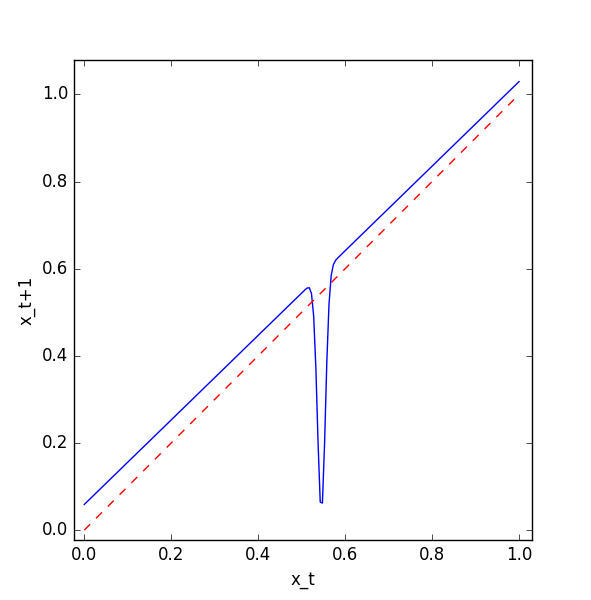
\includegraphics[width=\linewidth]{function_RBF_3.png}
  \caption{I = 1}
\endminipage\hfill
\minipage{0.32\textwidth}
  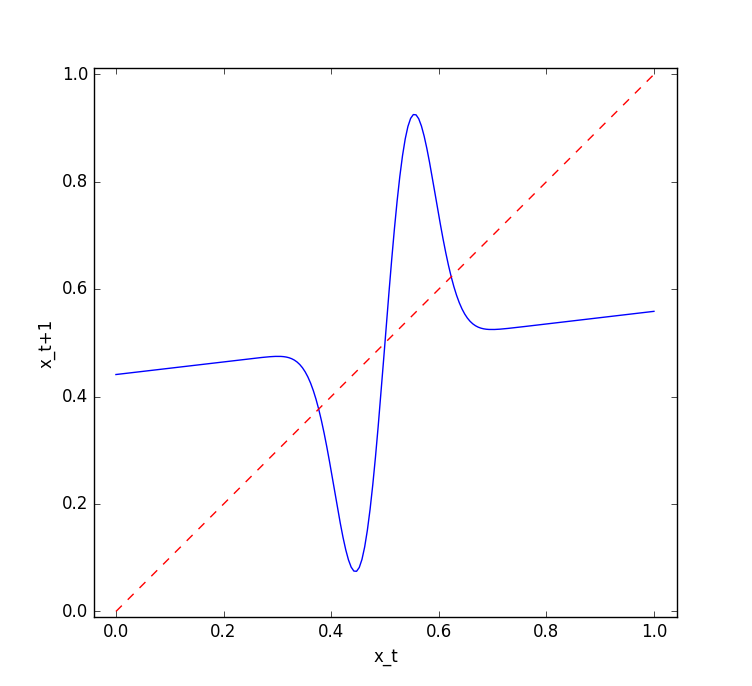
\includegraphics[width=\linewidth]{function_RBF_1.png}
  \caption{I = 2}
\endminipage\hfill
\minipage{0.32\textwidth}
  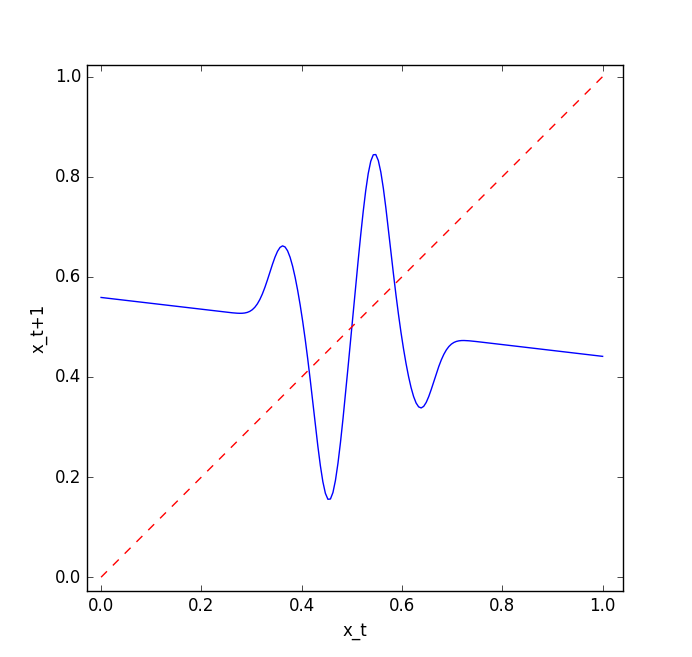
\includegraphics[width=\linewidth]{function_RBF_2.png}
  \caption{I = 4}
\endminipage\hfill
\end{figure}


\section{E-Step}

At iteration $k$, in the E-step, given the parameter $\theta^{(k-1)} = \left( \theta_f^{(k-1)}, \theta_g^{(k-1)}, Q^{(k-1)}, R^{(k-1)} \right)$ computed in the iteration $k-1$, we want to infer the sequences $(x_t)_{t=1 \ldots T}$ and $(x_t, x_{t+1})_{t=1 \ldots T-1}$ knowing the output sequence $(y_t)_{t=1 \cdots T}$ and the input sequence $(u_t)_{t=1 \cdots T}$.
In other words we want to compute the conditional probabilities :
\begin{align*}
  &p_{\theta^{(k-1)}}\left(x_t \given y_1, u_1, \ldots, y_T, u_T \right), t=1 \ldots T\\
  &p_{\theta^{(k-1)}}\left(x_t, x_{t+1} \given y_1, u_1, \ldots, y_T, u_T \right), t=1 \ldots T-1\\
\end{align*}

\textbf{Essentially we are able to solve this inference problem (filtering or smoothing) when the dynamic is linear.}
However,  if we use the non-linear dynamics equations with $f$ and $g$, we have no guarantees that, starting from a Gaussian probability for $x_1$, we will have a Gaussian probability for $x_{t}$, and the computations become intractable.
\textbf{To solve this problem, the authors propose to linearize the dynamics equations (\ref{eq:A},\ref{eq:B}) by their first order Taylor expansion at each time step $t$ and at a well-chosen point for filtering ($\tilde{x}_t$) and for smoothing ($\dot{x}_t$) :}
\begin{align*}
  x_{t+1} &= f(\tilde{x}_t, u_t) + A_{\tilde{x}_t} (x_t - \tilde{x}_t) + v_t\\
  A_t &= \frac{\partial f}{\partial x}(\tilde{x}_t, u_t)\\
  y_t &= g(\tilde{x}_t, u_t) + C_{\tilde{x}_t} (x_t - \tilde{x}_t) + w_t\\
  C_t &= \frac{\partial g}{\partial x}(\tilde{x}_t, u_t).\\
\end{align*}

Then the functions are locally linear, thus all probabilities are Gaussian and we can adapt the classical inferences algorithms (\textbf{Kalman filter} for filtering and \textbf{Rauch-Tung-Stribel smoother} for smoothing).\\

This forward-backward approach, involving a linearization at each time step, is called Extented Kalman Smoothing (EKS).
\textbf{One of the important issues is to define $\mathbf{\tilde{x}_t}$ and $\mathbf{\dot{x}_t}$.}

\subsection{Kalman filter}
Let's first recall how Kalman filter proceed with inputs. It is a particular case where $f$ and $g$ are affine (e.g. $I=0$ and $J=0$) :
\begin{align*}
  f(x,u) &= Ax + Bu + b\\
  g(x,u) &= Cx + Du + d\\
\end{align*}
the Kalman filter algorithm computes dynamically the conditional probabilities :
\begin{align*}
  &p_{\theta^{(k-1)}}\left(x_t \given y_1, u_1, \ldots, y_t, u_t \right), t=1 \ldots T\\
  &p_{\theta^{(k-1)}}\left(x_t, x_{t+1} \given y_1, u_1, \ldots, y_t, u_t \right), t=1 \ldots T-1\\
\end{align*}
Putting a gaussian probability on the first state $x_0$ and assuming the \textbf{additive} noise sequences $(w_t)$ and $(v_t)$ are Gaussian, since $f$ and $g$ are affine here, all the probabilities we are dealing with are then Gaussian.
Thus we only need to compute means and covariances.\\

The authors derive the computations of the Kalman filter only in the case where $B,b,D$ and $d$ are all zero.
They didn't give any reasons for these simplifications, but we extended the computations to take those into account.\\
%Is it lazyness?
%Is it intended for pedagoical reason?

As in \cite{Poly}, we denote by $\hat{x}_{t|t}$ the mean of $x_t$ conditioned on $u_1;\cdots;u_t$ and for $\hat{P}_{t|t}$ the covariance of $x_t$ given $u_1;\cdots;u_t$. It is straightforward to adapt these notations in the smoothing case ($\hat{P}_{t|T}$ and $\hat{x}_{t|T}$).
We adopt the following notations :
\begin{align*}
  \hat{x}_{t \given t} &= \mathbb{E}_p \left(x_t \given y_1, \ldots , y_t, u_1, \ldots , u_t \right) \\
  \hat{x}_{t+1 \given t} &= \mathbb{E}_p \left(x_{t+1} \given y_1, \ldots , y_t, u_1, \ldots , u_t \right) \\
  \hat{P}_{t \given t} &= \mathbb{E}_p \left((x_t - \hat{x}_{t \given t})(x_t - \hat{x}_{t \given t})^{\top} \given y_1, \ldots , y_t, u_1, \ldots , u_t \right) \\
  \hat{P}_{t+1 \given t} &= \mathbb{E}_p \left((x_{t+1} - \hat{x}_{t+1 \given t})(x_{t+1} - \hat{x}_{t+1 \given t})^{\top} \given y_1, \ldots , y_t, u_1, \ldots , u_t \right) \\
  \hat{P}_{t,t+1 \given t} &= \mathbb{E}_p \left((x_t - \hat{x}_{t \given t})(x_{t+1} - \hat{x}_{t+1 \given t})^{\top} \given y_1, \ldots , y_t, u_1, \ldots , u_t \right) \\
\end{align*}
As already mentioned, computing these quantities amounts to infer the conditional probability distribution of the hidden states since we are working with gaussians distribution. The Kalman filter gives us a recursion equation to compute these quantities :
\begin{itemize}
  \item \textbf{Initialization}\\
    \begin{align*}
      \hat{x}_{1 \given 0} &= 0\\
      \hat{P}_{1 \given 0} &= \Sigma_0\\
    \end{align*}
  \item \textbf{Forward recursion}\\
    For $t=1 \ldots T$ :
    \begin{align*}
      \hat{x}_{t+1 \given t} &= A \hat{x}_{t \given t} + B u_t + b\\
      \hat{P}_{t+1 \given t} &= A \hat{P}_{t \given t} A^{\top} + Q\\
      \hat{P}_{t,t+1 \given t} &= \hat{P}_{t \given t}A^{\top}\\
      K_{t+1} &= \hat{P}_{t+1 \given t}C^{\top}(C \hat{P}_{t+1 \given t} C^{\top} + R^{(k-1)})^{-1}\\
      \hat{x}_{t+1 \given t+1} &= x_{t+1 \given t} + K_{t+1} \left(y_{t+1} - (C\hat{x}_{t+1 \given t} + D u_t + d) \right)\\
      \hat{P}_{t+1 \given t+1} &= \hat{P}_{t+1 \given t} - K_{t+1} C \hat{P}_{t+1 \given t}\\
    \end{align*}
We compute the matrix $K_{t}$ (Kalman gain matrix) to simplify the computations.
\end{itemize}

In our case, $f$ and $g$ are not linear.
So for $t=1..T$ we linearize our functions $f$ and $g$ around the point $\tilde{x}_t$ and then we can apply the recursion equation below.
We define $\tilde{x}_t$ as following :
\begin{align*}
  \tilde{x}_1 &= \hat{x}_{1 \given 0}\\
  \tilde{x}_{t+1} &= f(\hat{x}_{t \given t}, u_t)\\
\end{align*}
Then, the dynamics become :
\begin{align*}
  A_t &= \frac{\partial f}{\partial x}(\tilde{x}_t, u_t) = A + \sum_{i=1}^I \rho_i(\tilde{x}_t) h_i (\tilde{x}_t - c_i)^{\top} S_i^{-1}\\
  C_t &= \frac{\partial g}{\partial x}(\tilde{x}_t, u_t) = C + \sum_{j=1}^J \rho'_j(\tilde{x}_t) k_j (\tilde{x}_t - c'_i)^{\top} {S'_j}^{-1}\\
  x_{t+1} &= A_{t} x_t + (f(\tilde{x}_t, u_t) - A_{t} \tilde{x}_t) + v_t\\
  y_t &= C_{t} x_t + (g(\tilde{x}_t, u_t) - C_{t}  \tilde{x}_t) + w_t\\
\end{align*}
in the recursion formula, we just have to replace the matrices $A$ and $C$ by the matrices $A_t$ and $C_t$  and we replace the vectors $b$ and $d$ by the vectors $b_t$ and $d_t$ :
\begin{align*}
  b_t &= f(\tilde{x}_t, u_t) - A_{\tilde{x}_t} \tilde{x}_t\\
  d_t &= g(\tilde{x}_t, u_t) - C_{\tilde{x}_t} \tilde{x}_t\\
\end{align*}
and we get the conditionnal probabilities of interest :
\begin{align*}
  &p_{\theta^{(k-1)}}\left(x_t \given y_1, u_1, \ldots, y_t, u_t \right), t=1 \ldots T\\
  &p_{\theta^{(k-1)}}\left(x_t, x_{t+1} \given y_1, u_1, \ldots, y_t, u_t \right), t=1 \ldots T-1\\
\end{align*}

\subsection{Rauch-Tung-Stribel smoother}
The authors provide no computations for the RTS.
So all the computations done here were inspired from the computations done in the lecture notes.

If the case where $f$ and $g$ are affine, the RTS smoother algorithm uses the conditionnal probabilities computed with Kalman filter to compute the conditional probabilities :
\begin{align*}
  &p_{\theta^{(k-1)}}\left(x_t \given y_1, u_1, \ldots, y_T, u_T \right), t=1 \ldots T\\
  &p_{\theta^{(k-1)}}\left(x_t, x_{t+1} \given y_1, u_1, \ldots, y_T, u_T \right), t=1 \ldots T-1\\
\end{align*}
Once again, theses probabilities are Gaussian and only we need to compute their means and covariances.

The following notations follow the same rule as for Kalman filtering:
\begin{align*}
  \hat{x}_{t \given T} &= \mathbb{E}_p(x_t \given y_1, \ldots , y_T, u_1, \ldots , u_T) \\
  \hat{P}_{t \given T} &= \mathbb{E}_p \left((x_t - \hat{x}_{t \given T})(x_t - \hat{x}_{t \given T})^{\top} \given y_1, \ldots , y_T, u_1, \ldots , u_T \right) \\
  \hat{P}_{t,t+1 \given T} &= \mathbb{E}_p \left((x_t - \hat{x}_{t \given T})(x_{t+1} - \hat{x}_{t+1 \given T})^{\top} \given y_1, \ldots , y_T, u_1, \ldots , u_T \right) \\
\end{align*}
With these quanities, we can compute the conditionnal probabilities of interest.
The Kalman filter gives us a recursion equation to compute these quanities :
\begin{itemize}
  \item \textbf{Initialization}\\
    For the initialization, we need to run a Kalman filter to get the quantities $\hat{x}_{t \given t}, \hat{P}_{t \given t}$ for $t=1 \ldots T$ and $\hat{x}_{t+1 \given t}, \hat{P}_{t+1 \given t}, \hat{P}_{t,t+1 \given t}$ for $t=a \ldots T-1$.
  \item \textbf{Backward recursion}\\
    For $t=T-1 \ldots 1$ :
    \begin{align*}
      L_t &= \hat{P}_{t \given t}A^{\top}\hat{P}_{t+1 \given t}^{-1}\\
      \hat{x}_{t \given T} &= \hat{x}_{t \given t} + L_t(\hat{x}_{t+1 \given T} - \hat{x}_{t+1 \given t})\\
      \hat{P}_{t \given T} &= \hat{P}_{t \given t} + L_t(\hat{P}_{t+1 \given T} - \hat{P}_{t+1 \given t})L_t^{\top}\\
      \hat{P}_{t,t+1 \given T} &= \hat{P}_{t,t+1 \given t} - (\hat{x}_{t \given t} - \hat{x}_{t \given T})(\hat{x}_{t+1 \given t} - \hat{x}_{t+1 \given T})^{\top}\\
    \end{align*}
    We compute the matrix $L_{t}$ to simplify the computations.
\end{itemize}

In our case, $f$ and $g$ are not linear.
We linearize them around the point $\dot{x}_t$ and then we can apply the recursion equation below.
We define  as follow :
\begin{align*}
  \dot{x}_t &= \hat{x}_{t \given t} = \mathbb{E}_p(x_t \given y_1, \ldots , y_t, u_1, \ldots , u_t) \\
\end{align*}
As we see, $\dot{x}_t$ can be seen as the mean of probability  $p_{\theta^{(k-1)}}\left(x_t \given y_1, u_1, \ldots, y_t, u_T \right)$ computed by the Kalman filter.
We also see that in the recursion forumla, the matrix $C$ and the vectors $b$ and $d$ do not appear.
So we just have to replace the matrix $A$ by the matrix $A_t$ :
\begin{align*}
  A_t &= \frac{\partial f}{\partial x}(\dot{x}_t, u_t)\\
\end{align*}
The computation of $A_t$ in term of our parameters $\theta_f^{(k-1)}$ and $\theta_g^{(k-1)}$ and of the centers and width of our RBF functions is the same as in the Kalman filter, replacing $\tilde{x}$ by $\dot{x}$.

So we end up with the means and covariance matrices of the probabilities
\begin{align*}
  &p_{\theta^{(k-1)}}\left(x_t \given y_1, u_1, \ldots, y_T, u_T \right), t=1 \ldots T\\
  &p_{\theta^{(k-1)}}\left(x_t, x_{t+1} \given y_1, u_1, \ldots, y_T, u_T \right), t=1 \ldots T-1\\
\end{align*}
\textbf{which are exactly what we wanted to compute during the E-step.
So we can move to the M-step.}


\section{M-step}

The article miss at providing a full understanding on how Radial basis functions are used to compute exactly the M-step. In order to implement safely, it is of interest to write down all the analytic computations. So let's start from the beginning:\\

At iteration $k$, in the M-step, we assume that the state sequence $(x_t)_{t=1 \ldots T}$ follow the probability $q \left(x_1, \ldots ,x_T \right)$ such that the state $x_t$ follow the Gaussian probability:
\begin{align*}
  q(x_t) = \mathcal{N}\left( \hat{x}_{t \given T}, \hat{P}_{t \given T} \right), \  t=1 \ldots T\\
\end{align*}
and that the joint states $(x_t, x_{t+1})$ follow the Gaussian probability:
\begin{align*}
  q(x_t, x_{t+1}) &=
  \mathcal{N}
    \left(
      \left[
        \begin{array}{c} \hat{x}_{t \given T} \\ \hat{x}_{t+1 \given T} \end{array}
      \right],
      \left[
        \begin{array}{cc} \hat{P}_{t \given T} & \hat{P}_{t,t+1 \given T}\\ \hat{P}_{t,t+1 \given T} & \hat{P}_{t+1 \given T} \end{array}
      \right]
    \right), \  t=1 \ldots T-1\\
\end{align*}
where the quantities the means $\hat{x}_{t \given T}$ and covariance matrices $\hat{P}_{t \given T}, \hat{P}_{t,t+1 \given T}$ were computed in the E-step.
We adopt the following notations:
\begin{align*}
  q_t(x) &= q(x = x_t)\\
  q_{t,t+1}(x,x') &= q \left((x,x') = (x_t, x_{t+1})\right)\\
\end{align*}

Now we want to compute the updated parameter $\theta^{(k)} = \left( \theta_f^{(k)}, \theta_g^{(k)}, Q^{(k)}, R^{(k)} \right)$.

The updated parameter $\theta^{(k)}$ is the maximizer of the expected complete likelihood $L_q$ which is equal to the maximizer of the expected complete log-likelihood $l_q$:
\begin{align*}
  \theta^{(k)} &= \underset{\theta}{\text{argmax }}L_q(\theta) = \underset{\theta}{\text{argmax }}l_q(\theta)\\
\end{align*}
First we need to express $l_q(\theta)$ using the graph factorization.
Our graphical model is the following :
\begin{figure}[H]
	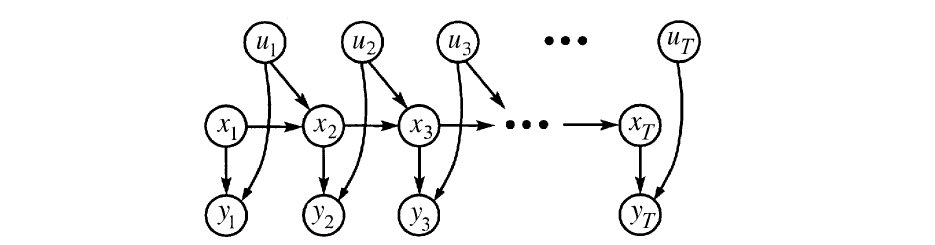
\includegraphics[width=14cm]{screenshot_graphical_model.PNG}
	\captionof{figure}{Graphical model of our system.}
\end{figure}
Firstly, the inputs $u_t$ are not modeled as random variable, so we won't take them into account in the factorization.
%\notes{If $u_t$ were random variables, we wouldn't have a tree anymore and the inference that we did in the E-Step would be complicated.}
Thus, the factorization over the graph yields :
\begin{align*}
p_{\theta}(x_1, \ldots x_T, y_1, \ldots , y_T) &= p_{\theta}(x_1) \prod_{t=1}^{T-1}{p_{\theta}(x_{t+1} \given x_t)} \prod_{t=1}^{T}{p_{\theta}(y_t \given x_t)}\\
\end{align*}
Thus, the likelihood of the observed the sequence $\overline{y} = (\overline{y}_t)_{t=1 \ldots T}$ is :
\begin{align*}
  p_{\theta}(x_1, \ldots x_T, \overline{y}_1, \ldots , \overline{y}_T) &= p_{\theta}(x_1) \prod_{t=1}^{T-1}{p_{\theta}(x_{t+1}\given x_t)} \prod_{t=1}^{T}{p_{\theta}(\overline{y}_t \given x_t)}\\
\end{align*}
Taking the $\log$ and expectation of this likelihood over the probability $q \left(x_1, \ldots ,x_T \right)$ gives us the expected log-likelihood:
\begin{align*}
  l_q(\theta) & =
    \mathbb{E}_q(\log(p_{\theta}(x_1))) +
    \sum_{t=1}^{T-1}{\mathbb{E}_q \left( \log(p_{\theta}(x_{t+1} \given x_t)) \right)} +
    \sum_{t=1}^{T}{\mathbb{E}_q\left( \log(p_{\theta}(\overline{y}_t \given x_t)) \right)}
  \\
  \mathbb{E}_q(\log(p_{\theta}(x_1))) &= -\frac{1}{2}\int_x{q_1(x) (x - \hat{x}_{1 \given 1})^{\top} \hat{P}_{1 \given 1}^{-1} (x - \hat{x}_{1 \given 1}) dx}
  \\
  \mathbb{E}_q \left( \log(p_{\theta}(x_{t+1} \given x_t)) \right) &= -\frac{1}{2}\int_{x,x'}{q_{t,t+1}(x, x') ((x' - f(x,u_t))^{\top} Q^{-1} (x' - f(x,u_t)) dxdx'}\\
  \mathbb{E}_q\left( \log(p_{\theta}(\overline{y}_t \given x_t)) \right) &= -\frac{1}{2}\int_x{q_t(x) (\overline{y}_t - g(x, u_t))^{\top} R^{-1} (\overline{y}_t - g(x, u_t)) dx}\\
\end{align*}
Firstly, to get rid of the multiplying constants $-\frac{1}{2}$, we multiply the expected log likelihood by $-2$ such that our maximization problem becomes a minimization problem :
\begin{align*}
  \theta^{(k)} &= \underset{\theta}{\text{argmin }}l(\theta)\\
\end{align*}
Then we notice that the expectation $\mathbb{E}_q(\log(p_{\theta}(x_1)))$ is constant with respect to $\theta$ so it doesn't account for the maximization.
Introducing the author notations :
\begin{align*}
  \Phi_f(x, u) &= [\rho_1(x), \ldots , \rho_I(x), x^{\top}, u^{\top}, 1]^{\top}\\
  \Phi_g(x, u) &= [\rho'_1(x), \ldots , \rho'_J(x), x^{\top}, u^{\top}, 1]^{\top}\\
  \left< F(.) \right>_{t} &= \int_x{q_t(x) F(x) dx} = \mathbb{E}_q \left( F(x_t) \right)\\
  \left< F(.) \right>_{t,t+1} &= \int_{x, x'}{q_{t,t+1}(x, x') F(x,x') dx}dx' = \mathbb{E}_q \left( F(x_t, x_{t+1}) \right)\\
\end{align*} % NOTA : on ne devrait pas avoir les mêmes x et u pour f et g
such that:
\begin{align*}
  f(x,u) = \theta_f \Phi_f(x, u)\\
  g(x,u) = \theta_g \Phi_g(x, u)\\
\end{align*}
and the functions $l^1_q$ and $l^2_q$:
\begin{align*}
  l^1_q(\theta_f, Q) &= \sum_{t=1}^{T-1}\left< (x, x') \mapsto (x' - \theta_f\Phi_f(x,u_t))^{\top} Q^{-1}(x' - \theta_f\Phi_f(x,u_t)) \right>_{t,t+1} + (T-1) \log( \given Q \given )
  \\
  l^2_q(\theta_g, R) &= \sum_{t=1}^{T}\left< x \mapsto (\overline{y}_{t} - \theta_g \Phi_g(x, u_t))^{\top} R^{-1} (\overline{y}_{t} - \theta_g \Phi_g(x, u_t)) \right>_{t} + T \log( \given R \given )
  \\
\end{align*}
our minimization problem becomes:
\begin{align*}
  \left(\theta_f^{(k)}, Q^{(k)}\right) &= \underset{\theta_k, Q}{\text{argmin }}l^1_q(\theta_f, Q)\\
  \left(\theta_g^{(k)}, R^{(k)}\right) &= \underset{\theta_g, R}{\text{argmin }}l^2_q(\theta_g, R)\\
\end{align*}
At the minimum point, the gradients vanish
\begin{align*}
  \left[
    \begin{array}{c} \nabla_{\theta_f} l^1_q \\ \nabla_{Q} l^1_q \end{array}
  \right] \left(\theta_f^{(k)}, Q^{(k)}\right) &=
  \left[
    \begin{array}{c} 0 \\ 0 \end{array}
  \right]\\
  \left[
    \begin{array}{c} \nabla_{\theta_g} l^2_q \\ \nabla_{R} l^2_q \end{array}
  \right] \left(\theta_g^{(k)}, R^{(k)} \right) &=
  \left[
    \begin{array}{c} 0 \\ 0 \end{array}
  \right] \\
\end{align*}
which yields:
\begin{align*}
  \theta_f^{(k)} &=
    \left(
      \sum_{t=1}^{T-1}{\left< x' \mapsto x' \Phi_f(x,u_t)^{\top} \right>_{t+1}}
    \right)
    \left(
      \sum_{t=1}^{T-1}{\left< x \mapsto \Phi_f(x, u_t)\Phi_f(x,u_t)^{\top} \right>_{t}}
    \right)^{-1}
  \\
  Q^{(k)} &=
    \frac{1}{T-1}
    \left(
      \sum_{t=1}^{T-1}{\left< x' \mapsto x'x'^{\top} \right>_{t+1}} -
      \theta_f^{(k)} \sum_{t=1}^{T-1}{\left< (x,x') \mapsto \Phi_f(x, u_t) x'^{\top} \right>_{t,t+1}}
    \right)
  \\
  \theta_g^{(k)} &=
    \left(
      \sum_{t=1}^{T}{\left< x \mapsto \overline{y}_{t}\Phi_g(x,u_t)^{\top} \right>_{t}}
    \right)
    \left(
      \sum_{t=1}^{T}{\left< x \mapsto \Phi_g(x,u_t)\Phi_g(x,u_t)^{\top} \right>_{t}}
    \right)^{-1}
  \\
  R^{(k)} &=
    \frac{1}{T}
    \left(
      \sum_{t=1}^{T}{\overline{y}_t \overline{y}_t^{\top}} -
      \theta_g^{(k)} \sum_{t=1}^{T}{\left< x \mapsto \Phi_f(x, u_t) \overline{y}_t^{\top} \right>_{t}}
    \right)
  \\
\end{align*}
Now the keypoint is to compute these expectations.
To compute $\theta_f^{(k)}$ and $Q^{(k)}$, we need to compute the expectations:
\begin{align*}
  \left< (x,x') \mapsto x' \Phi_f(x,u_t_t)^{\top} \right>_{t,t+1} &=
    \left< (x,x') \mapsto [x'\rho_1(x), \ldots , x'\rho_I(x), x'x^{\top}, x'u_t^{\top}, x']\right>_{t,t+1}
  \\
  \left< (x,x') \mapsto \Phi_f(x, u_t_t) x'^{\top} \right>_{t,t+1} &=
    \left< (x,x') \mapsto [x'\rho_1(x), \ldots , x'\rho_I(x), x'x^{\top}, x'u_t^{\top}, x']^{\top} \right>_{t,t+1}
  \\
  \left< x \mapsto \Phi_f(x, u_t_t)\Phi_f(x,u_t_t)^{\top} \right>_{t} &=
    \left< x \mapsto \left[
      \begin{array}{cccccc}
        \rho_1(x)\rho_1(x) & \ldots & \rho_1(x)\rho_I(x) & \rho_1(x)x^{\top} & \rho_1(x)u_t^{\top} & \rho_1(x) \\
        \ldots & \ldots & \ldots & \ldots & \ldots & \ldots\\
        \rho_I(x)\rho_1(x) & \ldots & \rho_I(x)\rho_I(x) & \rho_I(x)x^{\top} & \rho_I(x)u_t^{\top} & \rho_I(x) \\
        \rho_1(x)x & \ldots & \rho_I(x)x & xx^{\top} & xu_t^{\top} & x \\
        \rho_1(x)u_t & \ldots & \rho_I(x)u_t & u_t x^{\top} & u_tu_t^{\top} & u_t \\
        \rho_1(x) & \ldots & \rho_I(x) & x^{\top} & u_t^{\top} & 1 \\
      \end{array}
    \right]
  \right>_{t}
  \\
  \left< x' \mapsto x'x'^{\top} \right>_{t+1} &\\
\end{align*}
So we need to compute the elementary expectations:
\begin{align*}
  &\left< (x,x') \mapsto \rho_i(x) x' \right>_{t,t+1}\\
  &\left< (x,x') \mapsto x'x^{\top} \right>_{t,t+1}\\
  &\left< (x,x') \mapsto x' \right>_{t,t+1}\\
  &\left< x' \mapsto x'x'^{\top} \right>_{t+1}\\
  &\left< x \mapsto \rho_i(x)\rho_j(x) \right>_{t}\\
  &\left< x \mapsto \rho_i(x) x \right>_{t}\\
  &\left< x \mapsto \rho_i(x) \right>_{t}\\
  &\left< x \mapsto xx^{\top} \right>_{t}\\
  &\left< x \mapsto x \right>_{t}\\
\end{align*}
We begin with the simple ones :
\begin{align*}
  \left< x' \mapsto x'\right>_{t+1} &= \hat{x}_{t+1 \given T}\\
  \left< (x,x') \mapsto x'x^{\top}\right>_{t,t+1} &= \hat{x}_{t+1 \given T} \hat{x}_{t \given T}^{\top} + \hat{P}_{t,t+1 \given T}\\
  \left< x \mapsto xx^{\top}\right>_{t} &= \hat{x}_{t \given T} \hat{x}_{t \given T}^{\top} + \hat{P}_{t \given T}\\
  \left< x \mapsto x\right>_{t} &= \hat{x}_{t \given T}\\
\end{align*}
For the other expectations, the authors make us observe that when we multiply the RBF function $\rho_i$ and $q_t$, we obtain a Gaussian density in $\mathbb{R}^p$ with mean $\mu^i_t$ and covariance $\Sigma^i_t$ :
\begin{align*}
  \Sigma^i_t &= \left( \hat{P}_{t \given T}^{-1} + S_i^{-1} \right)^{-1}\\
  \mu^i_t &= \Sigma^i_t \left( \hat{P}_{t \given T}^{-1} \hat{x}_{t \given T} + S_i^{-1}c_i \right)\\
\end{align*}
multiplied by the constant $\beta^i_t$ (due to non-normalization):
\begin{align*}
  \beta^i_t &= (2\pi)^{-p/2} |S_i|^{-1/2} |\hat{P}_{t|T}|^{-1/2} |\Sigma^i_t|^{1/2} \exp(-\frac{1}{2} \delta^i_t)\\
  \delta^i_t &= c_i^{\top} S_i^{-1} c_i + \hat{x}_{t \given T}^{\top} \hat{P}_{t \given T}^{-1} \hat{x}_{t \given T} - {\mu^i_t}^{\top} \Sigma^i_t \mu^i_t\\
\end{align*}
Using these notations, the expectations involving $x_t$ and $\rho_i$ can be computed:
\begin{align*}
  \left< x \mapsto \rho_i(x) x \right>_{t} &= \beta^i_t \mu^i_t\\
  \left< x \mapsto \rho_i(x) \right>_{t} &= \beta^i_t\\
\end{align*}
Identically, when we multiply the product $\rho_i \rho_j$ and $q_t$, we obtain a Gaussian density in $\mathbb{R}^p$ with mean $\mu^{i,j}_t$ and covariance $\Sigma^{i,j}_t$ :
\begin{align*}
  \Sigma^{i,j}_t &= \left( \hat{P}_{t \given T}^{-1} + S_i^{-1} + S_j^{-1} \right)^{-1}\\
  \mu^{i,j}_t &= \Sigma^{i,j}_t \left( \hat{P}_{t \given T}^{-1} \hat{x}_{t \given T} + S_i^{-1}c_i + S_j^{-1}c_j \right)\\
\end{align*}
multiplied by the constant $\beta^{i,j}_t$ (due to non-normalization):
\begin{align*}
  \beta^{i,j}_t &= (2\pi)^{-p} |S_i|^{-1/2} |S_j|^{-1/2} |\hat{P}_{t|T}|^{-1/2} |\Sigma^{i,j}_t|^{1/2} \exp(-\frac{1}{2} \delta^{i,j}_t)\\
  \delta^{i,j}_t &= c_i^{\top} S_i^{-1} c_i + c_j^{\top} S_j^{-1} c_j + \hat{x}_{t \given T}^{\top} \hat{P}_{t \given T}^{-1} \hat{x}_{t \given T} - {\mu^{i,j}_t}^{\top} {\Sigma^{i,j}_t}^{-1} \mu^{i,j}_t\\
\end{align*}
and the expectation involving the product $\rho_i \rho_j$ is:
\begin{align*}
  \left< x \mapsto \rho_i(x)\rho_j(x)\right>_{t} &= \beta^{i,j}_t\\
\end{align*}
Finally, when we multiply the RBF function $\rho_i$ and $q_{t,t+1}$, we obtain a Gaussian density in $\mathbb{R}^{2p}$ with mean $\mu^i_{t,t+1}$ and covariance $\Sigma^i_{t,t+1}$ :
\begin{align*}
  \Sigma^i_{t,t+1} &=
    \left(
      \left[
        \begin{array}{cc} \hat{P}_{t \given T} & \hat{P}_{t,t+1 \given T}\\ \hat{P}_{t,t+1 \given T} & \hat{P}_{t+1 \given T} \end{array}
      \right]^{-1}
       +
      \left[
        \begin{array}{cc} S_i^{-1} & 0\\ 0 & 0 \end{array}
      \right]
    \right)^{-1}
  \\
  \mu^i_{t,t+1} =
    \left[
      \begin{array}{c} m^i_{t,t+1} \\ n^i_{t,t+1} \end{array}
    \right]
    &=
    \Sigma^i_{t,t+1}
      \left(
        \left[
          \begin{array}{cc} \hat{P}_{t \given T} & \hat{P}_{t,t+1 \given T}\\ \hat{P}_{t,t+1 \given T} & \hat{P}_{t+1 \given T} \end{array}
        \right]^{-1}
        \left[
          \begin{array}{c} \hat{x}_{t \given T} \\ \hat{x}_{t+1 \given T} \end{array}
        \right] +
        \left[
          \begin{array}{c} S_i^{-1}c_i \\ 0 \end{array}
        \right]
      \right)
  \\
\end{align*}
multiplied by a constant $\beta^{i}_{t,t+1}$ :
\begin{align*}
  \beta^i_{t,t+1} &= (2\pi)^{-p/2} |S_i|^{-1/2} |\hat{P}_{t|T}|^{-1/2} |\Sigma^i_{t,t+1}|^{1/2} \exp(-\frac{1}{2} \delta^i_{t,t+1})\\
  \delta^i_{t,t+1} &= c_i^{\top} S_i^{-1} c_i + \hat{x}_{t \given T}^{\top} \hat{P}_{t \given T}^{-1} \hat{x}_{t \given T} - {\mu^i_{t,t+1}}^{\top} {\Sigma^i_{t,t+1}}^{-1} \mu^i_{t,t+1}\\
\end{align*}
Thus the last expectation is :
\begin{align*}
  \left< (x,x') \mapsto \rho_i(x) x' \right>_{t,t+1} &= \beta^i_{t,t+1}n^i_{t,t+1}\\
\end{align*}

The interest of the RBF functions is that the expectations can be computed analytically and efficiently.
Otherwise, as soon as the state space dimension is big (for example $\geq 5$), these expectations must be estimmated, which is very expensive.


\section{The Initialization}

In our models we are faced with two kind of parameters. 
\begin{itemize}
\item \textbf{Hyper-parameters} are those that we are to set ourselves by build-out methods (cross-validation, selection criterion or home-made methods). In our case, $I_f$, $I_g$, $(c_i^f,S_i^f)$,$(c_i^g,S_i^g)$ and the dimension of the hidden variables are to be set. The article provides an heuristic way to set $(c_i^f,S_i^f)$ and $(c_i^g,S_i^g)$, that we will describe precisely.
\item \textbf{Parameters to be learned} are those that the EM-algorithm will output, e.g. $(\theta_f,\theta_g)$. \textbf{These parameters need to be initialized}. Note that the juncture between these two categories is quite porous. Indeed the centers and variances of the RBF Kernels could also be learn with an adaptive procedure inside the EM-algorithm. \textbf{Thus the setting of this parameters would become an initialization.}
\end{itemize}
Setting the Hyper-parameters is always a difficult issue, in particular in methods based of maximum-likelihood maximization because it cannot be used to discriminate the models.\\

\textbf{Also initialization of the parameters we want to learn is a crucial issue, especially for EM-algorithm that converges to local minima.} It is thus of interest to  start the algorithm with a good guess.\\



\subsection{Hyper-parameters:Fit the center and variance of RBF Kernel}
\textbf{Note that we will work with small (e.g. smaller than 4) for the dimension of the hidden variables.}\\



En fait ca c'est pour haute dimension, en petite il suffit de grider l'espace...(pas exactement clair)
\begin{enumerate}
\item First run the EM with linear dynamics (e.g. $x_{k+1}=Ax_k+B u_k +w_k$ and $y_k=C x_k + D u_k +v_k$). \textbf{don't know how to initialize it}.
\item Run the E-step with the parameters learn by the previous EM-algorithm.
\item Pick at random I means of the sequence of states. Check that they are not to close to one another. \textbf{Ici aussi ce n'est pas clair la distance prise}. If some are too close, pick new ones. These will be the given sequence for the centers of the RBF Kernel.
\item \textbf{Set the width (e.g. the variance matrix $S_i$) by "once we have the spacing of their centers by attempting to make neighbouring kernels cross when their outputs are half of their peak value."}
\end{enumerate}

\subsection{Initialization of $(\theta_g,\theta_f)$}
So we need to initialize the set of parameters (\textbf{Est-ce que Q et R y sont?}):
\begin{eqnarray*}
\theta_f &=& (f_1;\cdots;f_{I_f};A;B;b;Q)\\
\theta_g &=& (g_1;\cdots;g_{I_g};C;D;d;R)
\end{eqnarray*}

\subsubsection{First case}
Consider the case in which the dynamics is non-linear with approximately linear output function:
\begin{eqnarray}
x_{k+1} &=& \sum_{i=1}^{I_f}{f_i\rho_i(x_k)}+Ax_k+Bu_k+b+w_k\\\label{eq:caca}
y_{k} &=& Cx_k+Du_k+d+v_k\label{eq:Lin}
\end{eqnarray}
The steps of the initialization are:
\begin{itemize}
\item Approximate the dynamics in order to apply a factor analysis. Namely (\ref{eq:Lin}) is not changed, while we consider that $x_k$ follows $\mathcal{N}(0,R)$\notes{I don't understand why it is relevant}. Through an EM-algorithm, we come up with an estimate for $C$ and an estimate for the states.
\item Using regression to identify the $\theta_f$ parameters. 
\end{itemize}

\textbf{The factor analysis:} Consider that $x_k$ follows the law $\mathcal{N}(0,R)$ \notes{Not sure if we are compelled that they follow the same law/ follow essentially the law of $w_k$}. Then from (\ref{eq:Lin}) we have that $y_k|x_k\sim\mathcal{N}(Cx_k+Du_k+d,R)$. \notes{Note that in the coursework setting, $x_k\sim\mathcal{N}(0,I)$/ also Factor Analysis asks for R to be diagonal/ though was is important is that the EM estimation can be done correctly} \textbf{A developper: DEMANDE UN GROS BOULOT!!!}\\
T

\textbf{The regression step:} We can then try to find the set of parameters by regressing the state at time k by the state estimation at the previous time. For instance finding the parameters that minimize:
\begin{eqnarray}
\sum_{t=1}^{T-1}{\mathbb{E}(||x_{k+1}-x_k||^2)}&=&\sum_{t=1}^T{\mathbb{E}||\sum_{i=1}^{I_f}{h_i\rho_i(x_k)}+Ax_k+Bu_k+b+w_k-x_k||^2}
\end{eqnarray}
where the expectation is taken over the inferred distribution of $x_k$ in the factor analysis.

\subsubsection{Second case}
Now the case:
\begin{eqnarray}
x_{k+1} &=& Ax_k+Bu_k+w_k\\
y_{k} &=& \sum_{i=1}^{I_g}{g_i\rho_i(x_k)}+Cx_k+Du_k+d+v_k
\end{eqnarray}

\subsubsection{In the general case?}

\bibliography{biblio}

\end{document}
